\documentclass[t]{sdqbeamer}
%\documentclass[c]{sdqbeamer} 

\usepackage{listings}
\usepackage{graphicx}
\usepackage{tabularx}
\usepackage{multirow}
\usepackage{multicol}
\usepackage{tabulary}
\usepackage{colortbl}
\usepackage{tikzsymbols}
\usepackage{tikz}
\usetikzlibrary{positioning,fit,shapes}
\usepackage[lined,linesnumbered,ruled,noend]{algorithm2e}
\usepackage{bm}
\usepackage{enumitem}
\setlist[enumerate]{label*=\bf\alph*),ref=\alph*}
\setlist[itemize]{label=\textbullet}

\hypersetup{
	colorlinks=true,
	urlcolor=kit-orange
}

% set sdqbeamer options
\titleimage{blender-render}
\groupname{Algorithm Engineering}
\grouplogo{ae}
\selectlanguage{english}

% define title etc.pp.
\title[SAT Solving]{Practical SAT Solving}
\subtitle{Lecture 12}
\author{\underline{Markus Iser}, Dominik Schreiber, Tom\'a\v{s} Balyo}
\date{July 8, 2024}

% Existing KIT colors: kit-green, kit-blue, kit-red, kit-gray, kit-orange, kit-lightgreen, kit-brown, kit-purple, kit-cyan
% configure appearance
\setbeamercolor{block title}{bg=kit-blue}
\setbeamercolor{block body}{bg=kit-blue!10}
\setbeamercolor{block title example}{bg=kit-orange}
\setbeamercolor{block body example}{bg=kit-orange!10}
\setbeamertemplate{itemize item}{\color{kit-gray}\textbullet}
\setbeamertemplate{itemize subitem}{\color{kit-gray}\textbullet}
\setbeamercolor{item projected}{bg=kit-gray, fg=kit-gray}
\renewcommand{\insertnavigation}[1]{} % remove navigation bar

% define commands
\definecolor{myblue}{HTML}{0D3B66}
\definecolor{myred}{HTML}{6E0E0A}
\definecolor{mypink}{HTML}{F7B2B7}

\newcommand{\vars}[1]{\textsf{vars} (#1)}
\newcommand{\lits}[1]{\textsf{lits} (#1)}
\newcommand{\clss}[1]{\textsf{clss} (#1)}

\newcommand{\highl}[1]{\textcolor{myblue}{#1}}
\newcommand{\highlo}[1]{\textcolor{myred}{#1}}
\newcommand{\highlow}[1]{\textcolor{mypink}{#1}}

% Extra column types for tabularx
\newcolumntype{C}{>{\centering\arraybackslash}X}
\newcolumntype{L}{>{\raggedright\arraybackslash}X}
\newcolumntype{R}{>{\raggedleft\arraybackslash}X}

\newcommand{\setcolsep}[1]{\setlength{\tabcolsep}{#1}}
\newcommand{\setrowsep}[1]{\renewcommand{\arraystretch}{#1}}

% Definitions for the Tseitin transformation
\newcommand{\true}{\ensuremath{\mathit{True}}}
\newcommand{\false}{\ensuremath{\mathit{False}}}
\newcommand{\allvars}{\ensuremath{\mathcal{V}}}
\newcommand{\tseitin}[1]{\ensuremath{\mathcal{T}(#1)}}
\newcommand{\tseitinRec}[2]{\ensuremath{\mathcal{T}^{#2}(#1)}}
\newcommand{\tseitinSym}[1]{\ensuremath{\mathcal{T}_\mathsf{lit}(#1)}}
\newcommand{\tseitinDef}[2]{\ensuremath{\mathcal{T}_\mathsf{def}^{#2}(#1)}}
\newcommand{\hcancel}[2][black]{\setbox0=\hbox{$#2$}\rlap{\raisebox{.45\ht0}{\textcolor{#1}{\rule{\wd0}{1pt}}}}#2} 
\newcommand{\sateq}{\mathrel{\overset{\makebox[0pt]{\mbox{\normalfont\tiny\sffamily SAT}}}{=}}}

\newcommand{\enc}{\ensuremath{\mathcal{E}}} % encoding

% exercise commands
\newcommand{\exhead}[3]{
\hrule~\\[1ex]\noindent
{\bf Practical SAT Solving} (ST 2024) \hfill \fbox{Assignment #1} \\[1ex]
Markus Iser, Dominik Schreiber, Tom\'a\v{s} Balyo\\[1ex]
Algorithm Engineering (KIT) \hfill #2 -- #3\\
\hrule
\thispagestyle{empty}
}


\begin{document}
\begin{frame}
	\thispagestyle{empty}
	\titlepage
\end{frame}


\begin{frame}{Today: Preprocessing II and Proofs of Unsatisfiability}
    \begin{block}{Recap.}
    Preprocessing I (Lecture 7):
    \begin{itemize}
        \item Classic Preprocessing Techniques: Subsumption, Self-subsuming Resolution, Bounded Variable Elimination, Blocked Clause Elimination
        \item Relationship between Preprocessing Techniques and Gate Encodings
    \end{itemize}
    \end{block}
	\begin{block}{Today}
        \begin{itemize}
            \item Preprocessing II: Propagation-based Redundancy Notions
            \item Proofs of Unsatisfiabilty
        \end{itemize}
	\end{block}
\end{frame}
    

\begin{frame}{Preprocessing: Propagation-based Redundancy Notions}
Let a formula $F$, and a literal $x$ be given.
\begin{block}{Failed Literal Probing}
If $F \land x \vdash_{\mathop{UP}} \bot$, then $F \models \lnot x$\\[1ex]
$\implies$ add $\{ \lnot x \}$ to $F$
\end{block}
\begin{example}[Failed Literal Probing]
Let $F := \bigl\{ \{a, b\}, \{a, \lnot b\} \bigr\}$,\\[1ex]
then probing $\lnot a$ results in a conflict: $F \land \lnot a \vdash_{\mathop{UP}} \bot$,\\[1ex]
such that we can deduce $F \equiv F \land a$.
\end{example}
\end{frame}
    

\begin{frame}{Preprocessing: Propagation-based Redundancy Notions}
Let a formula $F$, a clause $C \in F$, and a literal $x \in C$ be given.
\begin{block}{Asymmetric Literal Elimination (ALE)}
If $F \setminus C \land \overline{C \setminus \{ x \}} \vdash_{\mathop{UP}} \overline x$, then $F \models C \setminus \{ x \}$.\\[1ex]
$\implies$ strengthen $C$ to $C \setminus \{ x \}$
\end{block}
\begin{example}[Asymmetric Literal Elimination (ALE)]
Let $F := \bigl\{ \{a, b\}, \{\lnot b, \lnot c\}, \{a, c, d\} \bigr\}$,\\[1ex]
and let $C := \{a, c, d\}$ and $x := c$,\\[1ex]
then $\bigl\{ \{a, b\}, \{\lnot b, \lnot c\}, \{\lnot a \}, \{\lnot d\} \bigr\} \vdash_{\mathop{UP}} \lnot c$,\\[1ex]
such that we can deduce $F \models \{a, d\}$.
\end{example}
$F$ can not have a model which satisfies $\{a, c, d\}$, but not $\{a, d\}$.
\end{frame}
    

\begin{frame}{Preprocessing: Propagation-based Redundancy Notions}
Let a formula $F$, a clause $C \in F$, and a literal $x \in C$ be given.
\begin{block}{Asymmetric Tautology Elimination (ATE)}
If $F \setminus C \land \overline C \vdash_{\mathop{UP}} \bot$, then $F \models C$.\\[1ex]
$\implies$ remove $C$ from $F$
\end{block}
\begin{example}[Asymmetric Tautology Elimination (ATE)]
Let $F := \bigl\{ \{a, b, c\}, \{\lnot b, d\}, \{a, c, d\} \bigr\}$,\\[1ex]
and let $C := \{a, c, d\}$,\\[1ex]
then $\bigl\{ \{a, b, c\}, \{\lnot b, d\}, \{\lnot a\}, \{\lnot c\}, \{\lnot d\}\} \bigr\} \vdash_{\mathop{UP}} \bot$,\\[1ex]
such that we can deduce $F \equiv F \setminus \{a,c,d\}$.
\end{example}
$\{a,c,d\}$ follows from the other clauses in $F$.
\end{frame}


\begin{frame}{Preprocessing: Propagation-based Redundancy Notions}
\begin{block}{Variants and Optimizations}~\\
\begin{itemize}\setlength{\itemsep}{1em}
    \item \textbf{Hidden Tautology Elimination (HTE) / Hidden Literal Elimination (HLE)}\\[1pt]
    Restricted forms of ATE/ALE which only propagate over binary clauses.
    \item \textbf{Distillation / Vivification}\\[1pt]
    Interleave assignment and propagation to detect ATs / ALs early on.
    \item \textbf{Avoidance of Redundant Propagations}\\[1pt]
    Sort literals and clauses in a formula to simulate a trie, and reuse propagations that share the same prefix.
    % \item \textbf{Unhiding}\footnote{\href{https://link.springer.com/chapter/10.1007/978-3-642-21581-0_17}{2011, Heule et al., Efficient CNF Simplification Based on Binary Implication Graphs}}\\[1pt] Avoid quadratic runtime of repeated unit propagation through randomized depth-first traversal of
    the binary implication graph and application of the \emph{parenthesis theorem}.
\end{itemize}~\\
\end{block}
\end{frame}

\begin{frame}{Preprocessing: Scheduling of Preprocessing Techniques}
At a point where one technique is unable to make further progress, another technique might be applicable and even modify the problem in a way that the first technique can make further progress.\\[1ex]

\begin{block}{Scheduling of Preprocessing Techniques}
\begin{itemize}\setlength{\itemsep}{1ex}
    \item \textbf{Heuristic Limits}\\[1pt]
    Bound the number of applications of a technique.
    \item \textbf{Scheduling of Techniques}\\[1pt]
    Non-trivial, benefit of techniques depends on the formula.
    \item \textbf{Interleaving of Techniques}\\[1pt]
    Apply techniques in a round-robin fashion.
    \item \textbf{Inprocessing}\\[1pt]
    Interleave search and preprocessing.
\end{itemize}
\end{block}
\end{frame}
    
\begin{frame}{Autarkies}
Let a formula $F$ and a partial assignment $A$ be given.\\[1ex]
\begin{itemize}\setlength{\itemsep}{1ex}
    \item A clause $C \in F$ is \highlo{touched} by $A$ if it contains the negation of a literal assigned in $A$
    \item A clause $C \in F$ is \highlo{satisfied} by $A$ if it contains a literal assigned to $\true$ by $A$
\end{itemize}
An autarky is a partial assignment $A$ such that \highlo{all touched clauses are satisfied}.
\begin{exampleblock}{Autarky}
The partial assignment $A = \{ \lnot a, \lnot c \}$ is an autarky for $F := \bigl\{\{ \lnot a, b \}, \{ \lnot a, c \}, \{ a, \lnot b, \lnot c \}\bigr\}$
\end{exampleblock}
\begin{block}{Autarky-based Clause Removal}
All clauses touched by an autarky can be removed.\\[1ex]
\textbf{Edge Case:} Pure Literals and Satisfying Assignments are Autarkies\\[1ex]
\textbf{Example Usage:} Kissat analyses assignments found by sprints of local search to find autarkies.
\end{block}
\end{frame}


\begin{frame}{Recap.}
\begin{block}{Preprocessing II}
    \begin{itemize}\setlength{\itemsep}{1em}
        \item Propagation-based Redundancy Notions: Failed Literal Probing, Asymmetric Literal Elimination, Asymmetric Tautology Elimination
        \item Autarkies: Partial assignments that satisfy all touched clauses
        \item Scheduling of Preprocessing Techniques
    \end{itemize}
\end{block}
\begin{block}{Next Up}
    Proofs of Unsatisfiability
\end{block}
\end{frame}

\begin{frame}{Relationship with Proof Checking}
\begin{block}{Generalizations of Blocked Clauses}~\\
\begin{itemize}\setlength{\itemsep}{1em}
    \item \textbf{Reverse Unit Propagation (RUP)}\\[1pt]
    A clause has the property RUP if and only if it is an Asymmetric Tautology (AT).\\[1ex]
    In CDCL, learned clauses are RUP at the moment of their learning.
    \item \textbf{Resolution Asymetric Tautologies (RATs)}\\[1pt]
    A clause $C$ is a RAT in a formula $F$ if it contains a literal $x$ such that \highlo{each resolvent in $C \otimes_x F_{\overline x}$ is an asymmetric tautology}.\\[1ex]
    Blocked Sets in particular are RATs.
\end{itemize}
~\\
\end{block}
\end{frame}


\begin{frame}{Proof Checking}
\vspace*{-1em}
SAT Solvers are complex software systems, and bugs are not uncommon.
\begin{block}{Trustworthiness of SAT Solvers}
The output of a SAT solver is trustworthy because:
\begin{itemize}\setlength{\itemsep}{1ex}
    \item For satisfiable instances, SAT solvers can output the found assignment
    \item For unsatisfiable instances, SAT solvers can output a proof of unsatisfiability
    \item Both can be checked independently from the solver by much simpler, and formally verified program
\end{itemize}
\textbf{Feasibility:} RAT proof checking is polynomial in the size of the proof, but the proof size is worst-case exponential in the size of the formula
\end{block}
\begin{example}[Applications]
Many real-world instances are unsatisfiable, e.g., unsatisfiability of a formula witnesses \dots
\begin{itemize}
    \item \dots the absence of certain bugs in a hardware design or software verification, 
    \item \dots or the optimality of a certain makespan in planning
    \item \dots  
\end{itemize} 
\end{example}
\end{frame}


\begin{frame}{Proof Systems: Motivating Example}
\begin{example}[Mutilated Chessboards]
Let a chessboard be given with two diagonally opposite corners removed.\\
Is it possible to cover the remaining board with dominoes?\\[1ex]
\visible<2>{\textbf{Human:} No, because each dominoe covers exactly one black and one white field, and there are two more black fields than white fields.}
\begin{center}

\includegraphics[width=.2\linewidth]{figures/l12/mcb0.png}
\end{center}
\end{example}
\end{frame}


\begin{frame}{Proof Systems: Motivating Example}
\begin{example}[Mutilated Chessboards]
Let a chessboard be given with two diagonally opposite corners removed.\\
Is it possible to cover the remaining board with dominoes?\\[1ex]
\textbf{SAT Solver:} Let's try and learn.\\
\begin{tabularx}{\linewidth}{XXX}
    
\includegraphics[width=.8\linewidth]{figures/l12/mcb1.png} &
    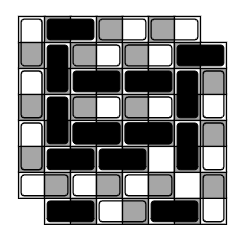
\includegraphics[width=.8\linewidth]{figures/l12/mcb2.png} &
    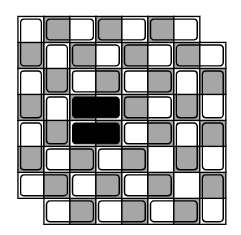
\includegraphics[width=.8\linewidth]{figures/l12/mcb3.png}\\
    \hline
    Impasse Detected & $\rightarrow$ Resolution & $\rightarrow$ More powerful Proof-system
\end{tabularx}
\end{example}
\end{frame}


\begin{frame}{Proof Complexity}
Proof complexity is the study of the size of proofs in different proof systems.\\[1ex]
\begin{block}{Relationship with SAT Solving}
\begin{itemize}\setlength{\itemsep}{1ex}
\item Static analysis without algorithmic considerations
\item Questions of automizability not addressed
\item Lower bounds on proof size tell us how good a SAT solver can be in the best case 
\item Upper bounds on proof size tell us how good a SAT solver should be
\end{itemize}
\end{block}
\end{frame}


\begin{frame}{Resolution vs. Extended Resolution}
\begin{block}{Resolution}
\begin{itemize}\setlength{\itemsep}{1ex}
    \item Preserves equivalence
    \item CDCL is as powerful as General Resolution
    \item Exponential Lower Bounds: For example, proofs of unsatisfiabilty of Pigeon Hole formulas, are necessarily of exponential length in the resolution proof system (Haken 1985)
\end{itemize}
\end{block}
\begin{block}{Extended Resolution (ER)}
\begin{itemize}\setlength{\itemsep}{1ex}
    \item Preserves satisfiability
    \item Extended Resolution (Tseitin 1966):\\
    incorporate extension rule $x \leftrightarrow a \land b$ for some $a,b$ in formula and a new variable $x$
    \item No Lower Bounds known
    \item (Cook 1967) polynomial sized ER proof for PH formulas
\end{itemize}
\end{block}
\end{frame}


\begin{frame}{Blocked Clauses (Kullmann 1999)}
\begin{block}{Blocked Clauses}
\begin{itemize}\setlength{\itemsep}{1ex}
    \item Preserves satisfiability
    \item Generalization of ER Proof systems
    \item Allows the addition and removal of blocked clauses
    \item No Lower Bounds known
\end{itemize}
\end{block}
\pause
\begin{block}{Problem: Automizability, how to find such short proofs?}
Structural Boundend Variable Addiction (SBVA) $\rightarrow$ SBVA CaDiCaL
\begin{itemize}\setlength{\itemsep}{1ex}
    \item Select variables based on their centrality in the Variable Interaction Graph (VIG) of the formula, then add definitions over these variables in a preprocessing step
    \item Winner of the Main track of SAT Competition 2023
    \item First time in history of SAT competitions that a heuristic for ER could beat CDCL
\end{itemize}
\end{block}
\end{frame}


\begin{frame}{Strong Proof-Systems without Introducing Variables}
\vspace*{-1em}
ER introduces new variables. Can we get stronger without introducing new variables?\\
In the following: $C$ is redundant with respect to $F$ means that $F$ and $F \land C$ are equisatisfiable.
\begin{example}[Implication-based Redundancy]
Given $F := \{\{x, y, z\}, \{\lnot x, y, z\}, \{x, \lnot y, z\}, \{\lnot x, \lnot y, z\}\}$, and $G := \{\{z\}\}$, \\
$G$ is at least as satisfiable as $F$ since $F \models G$
\end{example}
\pause
\begin{block}{Implication-based Redundancy Notion}
A clause $C$ is redundant w.r.t. formula $F$ iff there exists an assignment $\omega$ such that $F \land \lnot C \models (F \land C)|_\omega$%
\footnote{Given an assignment $\alpha$, the formula $F|_\alpha$ is the formula after removing from $F$ all clauses that are satisfied and all literals falsified by $\alpha$}
~\\[1ex]
\textbf{In other words:} Potential models of $F$ falsifiying $C$ are still models of $F$ and $C$ modulo an assignment $\omega$
\end{block}
\pause
\begin{block}{In Practice: Propagation Redundancy}
Approximate $F \land \lnot C \models (F \land C)|_\omega$ with unit propagation: $F \land \lnot C \vdash_{UP} (F \land C)|_\omega$\\
$\rightarrow$ Efficiently Checkable Proofs: \href{https://cakeml.org/tacas21.pdf}{Tan et al., Verified Propagation Redundancy Checking in CakeML, TACAS 21}
\end{block}
\end{frame}


\begin{frame}{Theorem: Clause Redundancy via Implication}
\vspace*{-2ex}
Let F be a formula, C a non-empty clause, and $\alpha$ the assignment blocked by C. Then, C is redundant with respect to F if and only if there exists an assignment $\omega$ such that $\omega$ satisfies C and $F|_\alpha \models F|_\omega$.\\
\hfill(\href{https://doi.org/10.1007/s10817-019-09516-0}{Heule et al., 2019, Strong Extension-Free Proof Systems})

\begin{block}<only@1>{\textbf{Proof ``only if''}}
\highl{Assume $F$ and $F \land C$ are equisatisfiable.} \highlo{Show that there exists an $\omega$ satisfying $C$ and $F|_\alpha \models F|_\omega$.}\\[1ex]
If $F|_\alpha$ is unsatisfiable, then the semantic implication trivially holds.\\[1ex]
Assume now that $F|_\alpha$ is satisfiable, implying that F is satisfiable.\\
Since $F$ and $F \land C$ are equisatisfiable, there exists an assignment $\omega$ that satisfies both $F$ and $C$.\\
Thus, since $\omega$ satisfies F, it holds that $F|_\omega = \emptyset$ and so $F|_\alpha \models F|_\omega$.
\end{block}

\begin{block}<2>{\textbf{Proof ``if''}}
\highl{Assume there exists an assignment $\omega$ satisfying $C$ and $F|_\alpha \models F|_\omega$.} \highlo{Show that $F$ and $F \land C$ are equisatisfiable.}\\[1ex]
Let $\gamma$ be a (total) assignment that satisfies $F$ and falsifies $C$. Then, we can turn $\gamma$ into a satisfying assignment $\gamma'$ for $F \land C$ as follows:\\
As $\gamma$ falsifies $C$, it coincides with $\alpha$ on \vars{C}. Therefore, since $\gamma$ satisfies $F$, it must satisfy $F|_\alpha$ and since $F|_\alpha \models F|_\omega$, it must also satisfy $F|_\omega$.
Now, consider the following assignment $\gamma'$ which clearly satisfies $C$:
$$
\gamma'(x) = \begin{cases} 
    \omega(x) & \text{if } x \in \vars{\omega}\\ 
    \gamma(x) & \text{otherwise}
\end{cases}
$$
Since $\gamma$ satisfies $F|_\omega$, and $\vars{F|_\omega} \subseteq \vars{\gamma} \setminus \vars{\omega}$, $\gamma'$ satisfies $F$.
Hence, $\gamma'$ satisfies $F \land C$.
\end{block}
\end{frame}


\begin{frame}{Pruning Branches with Conditional Autarkies}
\textbf{Theorem (Monien and Speckenmeyer 1985):}
Let $\alpha$ be an autarky of $F$. Then, $F$ and $F|_\alpha$ are equisatisfiable.\\[1ex]

\begin{block}{Conditional Autarkies}
An assignment $\alpha = \alpha_{con} \cup \alpha_{aut}$ is a conditional autarky of $F$ if $\alpha_{aut}$ is an autarky of $F|_{\alpha_{con}}$\\[1ex]
Then $F$ and $F \land (\alpha_{con} \rightarrow \alpha_{aut})$ are equisatisfiable.\\[1ex]
\end{block}
\begin{example}[Pruning Branches with a Conditional Autarky]
Let $F := \{\{x, y\}, \{x, \lnot y\}, \{\lnot y, \lnot z\}\}$, and let $\alpha_{con} = \{x\}$ and $\alpha_{aut} = \{\lnot y\}$.\\[1ex]
Then $F|_{\alpha_{con}} = \{\lnot y, \lnot z\}$ and $\alpha_{aut} = \{\lnot y\}$ is an autarky of $F|_{\alpha_{con}}$,\\ such that $\alpha = \{x, \lnot y\}$ is a conditional autarky of $F$.\\[1ex]
We can thus learn the clause $\{\lnot x, \lnot y\}$.
\end{example}
\end{frame}


\begin{frame}{Satisfaction Driven Clause Learning (SDCL)}
\textbf{Idea:} Also learn clauses if no conflict is detected, but a positive reduct is satisfiable.\\[1ex]

\begin{block}{Positive Reduct}
Let $\alpha := \lnot C$, the positive reduct $p(F, \alpha)$ is the formula that contains $C$ and all clauses of $F$ satisfied by $\alpha$.\\[1ex]
A satisfying assignment $\omega$ of the positive reduct $p(F,\alpha)$ is a conditional autarky of $F$.\\[1em]
Positive reducts are typically very easy to solve.
\end{block}
\textbf{Key Idea of SDCL:} While solving a formula, check the positive reducts of current assignments $\alpha$ for satisfiability, and if so, prune the branch $\alpha$.\\[1em]
\href{https://doi.org/10.1007/978-3-319-70389-3_12}{Heule et al., 2017, PRuning Through Satisfaction}
\end{frame}


\begin{frame}{Last slide}
\begin{block}{Recap.}
\begin{itemize}\setlength{\itemsep}{1em}
    \item Preprocessing II: Propagation-based Redundancy Notions, Autarkies, Scheduling of Preprocessing Techniques
    \item Proof Systems: Resolution, Extended Resolution, Blocked Clauses, Implication-based Redundancy
    \item Pruning Branches with Conditional Autarkies
    \item Satisfaction Driven Clause Learning (SDCL)
\end{itemize}
\end{block}
\end{frame}

% \begin{frame}{From Modern to Post-modern SAT Solving}
% \begin{block}{Next Time}
% \begin{itemize}\setlength{\itemsep}{1em}
% \item \textbf{Resolution Calculus} (a.k.a. Clause Learning)
% \item \textbf{Tseitin's Extension Rule}: Introduce definitions of new variables as a conjunction of existing literals (a.k.a. Bounded Variable Addition (BVA)). Some formulas have refutations of exponential size in the resolution calculus, but of polynomial size in extended resolution, e.g., pigeonhole formulas, mutilated chessboard, \dots\\[1ex]
% $\bm\rightarrow$ \texttt{SBVA-CaDiCaL}: Winner of SAT Competition 2023
% \item \textbf{PReLearning}: Preprocessing adds specific Propagation Redundant (PR) clauses\\[1ex]
% $\bm\rightarrow$ \texttt{KissatMAB-Prop}: Winner of SAT Competition 2023 on UNSAT instances
% \item \textbf{Symmetry Breaking Predicates}: Exclusion of Symmetric Solutions\\[1ex]
% $\bm\rightarrow$ \texttt{BreakId-Kissat}: Special Price at SAT Competition 2023
% \end{itemize}
% \end{block}
% \end{frame}

\end{document}
